% !TEX program = xelatex
\documentclass[UTF8,a4paper,11pt,fontset=none]{ctexart}
\usepackage[margin=2.05cm,headheight=16pt,headsep=10pt]{geometry}
\usepackage{fontspec}
\setmainfont{Times New Roman}
\setsansfont{Arial}
\setmonofont{Menlo}[Scale=.88]
\setCJKmainfont{Songti SC}[BoldFont=Songti SC Bold]
\setCJKsansfont{Heiti SC}
\setCJKmonofont{Heiti SC}
\usepackage{amsmath,amssymb,mathtools,booktabs,array,tabularx,longtable,multirow}
\usepackage{graphicx,xcolor,colortbl,caption,subcaption,float,enumitem,microtype}
\usepackage[sort&compress,numbers]{natbib}
\usepackage{fancyhdr,lastpage,placeins}
\usepackage[colorlinks=true,linkcolor=blue!45!black,citecolor=blue!45!black,urlcolor=blue!50!black,breaklinks=true]{hyperref}
\definecolor{ink}{HTML}{283741}\definecolor{accent}{HTML}{547B7D}\definecolor{pale}{HTML}{EFF4F3}
\pagestyle{fancy}\fancyhf{}\fancyhead[L]{\small 面向数学公式的专用分词}\fancyhead[R]{\small 内在质量与四类泛化实验}\fancyfoot[C]{\small\thepage}
\renewcommand{\headrulewidth}{.3pt}
\setlength{\parindent}{2em}\setlength{\parskip}{2pt}\linespread{1.12}
\setlength{\emergencystretch}{2em}
\ctexset{section={format=\large\bfseries,beforeskip=14pt,afterskip=7pt},subsection={format=\normalsize\bfseries,beforeskip=10pt,afterskip=5pt}}
\setlist{nosep,leftmargin=2em,topsep=3pt}
\captionsetup{font=small,labelfont=bf,labelsep=quad}
\captionsetup[table]{position=top,skip=5pt}
\setlength{\tabcolsep}{4.5pt}\renewcommand{\arraystretch}{1.13}
\newcommand{\code}[1]{\texttt{\detokenize{#1}}}
\newcommand{\up}{\ensuremath{\uparrow}}\newcommand{\dn}{\ensuremath{\downarrow}}
\newcommand{\mib}{\ensuremath{\mathrm{MiB/s}}}
\newcolumntype{Y}{>{\raggedright\arraybackslash}X}
\begin{document}
\thispagestyle{empty}
\noindent\textcolor{accent}{\small 数学语料与分词器研究\hfill 2026年10月15日}
\vspace{5pt}\hrule\vspace{15pt}
\begin{center}
{\LARGE\bfseries 面向数学公式的专用分词：\\[6pt]硬／软 AST 约束与四类泛化实验}\par
\vspace{10pt}{\normalsize 肖童仁}\par
\vspace{4pt}{\small Design and Evaluation of Specialized Tokenizers for Mathematical Formulas}
\end{center}
\vspace{8pt}\hrule\vspace{9pt}
\noindent\begin{minipage}[t]{.23\linewidth}
\textbf{研究信息}\par\smallskip\small
数学公式分词\par 抽象语法树\par 子词词表\par 跨领域泛化\par 可逆编码\par
\medskip\textbf{代码与数据}\par\smallskip
\href{https://github.com/xtr1976536/math-tokenizer-lab}{math-tokenizer-lab}\par
\medskip\textbf{实验规模}\par\smallskip
56,000条公式\par 9个分词器\par 11组划分\par 8项评价指标
\end{minipage}\hfill\begin{minipage}[t]{.72\linewidth}
\textbf{摘\quad 要}\par\smallskip
本文在56,000条研究级LaTeX公式上比较数学专用分词与通用分词。固定训练型模型词表为1,024，评价标准硬AST-BPE、AST-v4、Boundary AST和Math-atom BPE，并与Byte BPE、SentencePiece Unigram、Qwen2.5、Llama 3及o200k比较。实验设置全领域新来源、整域留出、分析方程与代数双向迁移、简单到复杂四类测试，共11组划分和99组模型评价。统一测量T/B、命令完整性、数字词素完整性、编码速度、Used、Cross、复合AST节点对齐率与Rényi效率。全领域测试中，Boundary AST相对Byte BPE减少7.45\%的每字节token数，Cmd为99.73\%；AST-v4的复合节点对齐率为73.33\%，编码速度为32.42 MiB/s。硬结构约束、软结构代价与数学词法原子分别形成不同的压缩、对齐和效率表现。全部评价通过逐式可逆性检验，并提供完整划分、逐式记录与五轮审查。

\end{minipage}
\vspace{10pt}\hrule\vspace{9pt}
\section{研究问题与相关工作}
数学公式由控制命令、数字、运算符、变量和层次化参数组构成。通用分词器通常依据文本频率构建子词，而数学专用分词可以额外使用词法原子或语法树信号。本文研究三个问题：在固定1,024个ID的条件下，数学原子能否提高编码压缩与命令完整性；AST硬约束与软约束如何改变压缩、结构对齐和速度；这些性质能否迁移到新来源、新领域以及更复杂的公式。

分词器的设计包含基础单位、词表学习和推理分割三个环节。Sennrich等\citep{sennrich-etal-2016-neural}将BPE用于开放词表建模；Kudo\citep{kudo-2018-subword}提出Unigram子词模型，SentencePiece\citep{kudo-richardson-2018-sentencepiece}将原始字符串训练与分词接口统一起来。Müller和Vlachos\citep{muller2019ast}提出AST-BPE，按照语法树限制可合并的相邻节点。AST-T5\citep{gong2024ast}进一步说明，结构树既可用于分割，也可用于预训练目标。本文将硬约束AST-BPE迁移到数学公式，并与保留硬约束的AST-v4和采用软代价的Boundary AST进行比较。

评价方面，压缩长度、词表分布和结构对齐测量不同性质。Zouhar等\citep{zouhar-etal-2023-tokenization}用Rényi熵衡量词表信道效率；Uzan等\citep{uzan-etal-2024-greed}区分词表构造与推理算法的作用；Schmidt等\citep{schmidt-etal-2024-tokenization}和Lotz等\citep{lotz-etal-2025-beyond}分别从受控预训练和跨规模评价研究压缩以外的分词性质。TokEval\citep{meister2026tokeval}同时覆盖压缩、词表利用率、速度和语法节点对齐。本文保留六项既有指标，增加Rényi效率和复合AST节点对齐率，形成八项评价。

数学数字的切分还涉及位值和算法对齐。Singh和Strouse\citep{singh2024counts}以及NumeroLogic\citep{schwartz-etal-2024-numerologic}研究了数字表示与算术任务之间的关系。本文的Num专门测量源码连续数字词素是否被切开；与其互补的数学推理与方程求解，将在后续语言模型实验中检验。不同指标各自对应清晰的观测对象，结果按指标分别比较。

\section{数学公式数据集}
\subsection{来源、内容与类别}
数据集包含56,000条LaTeX公式，来自366个来源组：283篇历史arXiv论文、11篇公开仓库论文及72个FunGrim／SymPy资源模块。每条记录保存公式、来源论文或资源、固定版本、许可、原始位置、变换记录、内容哈希、领域、复杂度和独立KaTeX语法跨度。评估使用目录中保存的原字符串，编码与解码均不改变空格、换行或命令拼写。

\begin{table}[htbp]\centering\small
\caption{语料来源。来源标签与数学领域分别存储。}\label{tab:sources}
\begin{tabularx}{\linewidth}{Y r Y l}\toprule
来源&公式数&版本与来源标签&许可\\\midrule
\href{https://arxiv.org/}{2020年前arXiv论文}&51,229&283个固定历史论文来源；human&CC BY／CC0\\
\href{https://github.com/openai/math/tree/fd4aeeb2ee4fc729c18d98444fed42fd0529eeeb}{OpenAI数学仓库}&2,810&固定Git版本；possible\_mixed&Apache-2.0\\
\href{https://github.com/fredrik-johansson/fungrim/tree/b7c3ca6e565e1058638cab6ba2bc811090296767}{FunGrim}&1,889&固定资源版本；unknown&MIT\\
\href{https://github.com/sympy/sympy/tree/sympy-1.10}{SymPy}&72&固定资源版本；unknown&BSD\\\midrule
合计&56,000&366个来源组&逐条记录\\\bottomrule
\end{tabularx}
\end{table}

来源构建依次进行：获取固定版本源文件，提取数学环境，展开记录中的局部宏，验证公式语法和宏变换前后的渲染一致性，去重，登记来源与许可，完成分类，保存公式和元数据。\code{human}依据2020年前论文版本及作者信息登记；其余来源分别使用\code{possible_mixed}和\code{unknown}标签。原始公式、宏定义和展开后的评估字符串可以相互追溯。

\begin{table}[htbp]\centering\small\caption{领域分布：公式领域与来源论文领域分别计数。}\label{tab:domains}\begin{tabular}{lrr@{\qquad}lrr}\toprule 领域&公式领域&论文领域&领域&公式领域&论文领域\\\midrule
分析 & 20,233 & 9,723 & 概率 & 3,171 & 3,171 \\
几何与拓扑 & 9,135 & 9,185 & 统计 & 1,056 & 1,056 \\
组合 & 5,563 & 5,563 & 逻辑 & 662 & 662 \\
代数 & 4,431 & 4,431 & PDE & 356 & 5,758 \\
数论 & 4,273 & 4,273 & ODE & 46 & 5,100 \\
数学物理 & 3,850 & 3,850 & 线性代数 & 13 & 13 \\
优化 & 3,211 & 3,215 &  &  &  \\
\bottomrule\end{tabular}\end{table}


公式领域与论文领域采用两个字段。前者按照公式本身的微分关系和结构分类；后者记录来源论文的学科，用于整域留出。严格PDE公式共356条，ODE公式46条。结构标签允许一式多类，包括恒等式或界、求和或乘积、积分、矩阵、多行公式、微分关系和方程组。领域划分使用论文领域，因而来自PDE论文中的积分或代数表达式仍属于PDE来源域。

\subsection{复杂度定义与集合隔离}
句法复杂度综合公式长度和符号复杂度。令$L$为LaTeX词素数、$C$为命令种类、$D$为嵌套深度、$S$为符号种类、$O$为运算符数，则
\begin{equation}\label{eq:complexity}
\begin{split}
K(x)={}&.40\min(L/60,2)+.20\min(C/6,2)\\
&+.15\min(D/3,2)+.15\min(S/18,2)+.10\min(O/12,2).
\end{split}
\end{equation}
$K(x)<.65$标记为简单，$K(x)\geq.65$标记为复杂。目录中简单公式37,400条，复杂公式18,600条。该分类测量源码句法复杂度。例如，公式ID\code{00023ce032027f7126dc1db0}的$(L,C,D,S,O)=(38,4,2,14,5)$，对应$K=0.645$，归入简单类。


本轮根据固定随机种子生成新的研究划分，保存每一集合的全部公式ID。首先在论文或资源模块层面分组，再删除训练、验证与测试之间的模板和MathML渲染重复。训练集合优先保留；验证集合删除与训练重复的项；测试集合删除与训练或验证重复的项。三者的公式ID、来源组、模板哈希及渲染哈希均无交集。

\section{比较模型与严格定义}
记输入的UTF-8字节串为$x$，词表为$V$，编码结果为$z=(z_1,\ldots,z_T)$。每个token对应原串的连续字节片段，解码为这些片段按序拼接。六个在本数据集上训练的模型均使用恰好1,024个ID，基础字节与预留原子均计入总数。三个通用分词器使用原始官方词表和代码接口。所有模型编码同一批原始公式，不添加BOS、EOS或对话模板。

\subsection{标准硬AST-BPE：受语法约束的逐次合并}
标准AST-BPE遵循Müller和Vlachos\citep{muller2019ast}的约束合并原则。本文将SQL场景迁移到LaTeX：叶节点保留源码位置，叶内部以字节表示，训练只统计与语法层次兼容的相邻片段。数学前端支持算术优先级、分式、根式、分组和上下标；其他LaTeX结构采用命令与参数的绑定语法树。

设候选token区间为$[a,b)$，参考节点区间为$[u,v)$。若满足
\begin{equation}\label{eq:cross}
a<u<b<v\quad\text{或}\quad u<a<v<b,
\end{equation}
两者发生部分跨越。硬约束要求候选区间与所有前端节点均不发生式\eqref{eq:cross}的关系。训练按合法相邻对的频率选择合并，记录有序合并规则，直至词表达到1,024。推理从字节出发，依照训练合并顺序执行当前合法的合并。该模型不预留数学命令原子，完整命令通过BPE学习。

\subsection{AST-v4：数学原子初始化与硬约束最短分割}
AST-v4沿用硬AST主线，在训练前从训练公式中选取至多256个高频控制命令和非ASCII字符作为原子；加上256个基础字节后，余下预算用于受AST约束的BPE合并。原子按训练频率排序，同频时按字节排序。推理在原串上构建词表匹配格，删除跨越前端语法节点或切开已覆盖完整命令的候选边，再求
\begin{equation}\label{eq:harddp}
z^*=\arg\min_{z\in\mathcal Z_{\mathrm{hard}}(x;V)}|z|.
\end{equation}
动态规划从右向左计算最少token路径。与标准硬AST-BPE相比，v4保留训练期与推理期的硬结构约束，增加数学原子初始化，并用完整词表上的最短路径替代逐次合并推理。原生C前端、trie匹配和动态规划在一次编码调用内完成。

\subsection{Math-atom BPE：数学原子上的标准BPE}
Math-atom BPE首先从训练集选取至多384个高频完整控制命令和非ASCII字符，与256个基础字节构成可逆原子字母表。已登记的完整命令映射成单个基础符号，其内部不允许出现切点；其他输入以字节表示。然后直接使用Hugging Face官方BPE训练和推理，学习合并到1,024个ID。该方法的数学信号位于基础字母表，BPE合并本身采用官方实现。

\subsection{Boundary AST：共享词表与软结构代价}
Boundary AST与Math-atom BPE共享同一训练所得词表。其命令原子约束保持不变，语法树约束改为可累计的软代价。令$C_{\mathrm{native}}(z,x)$为与推理前端语法跨度发生部分跨越的token数，$G(x)$为非空花括号组的内部内容端点集合，$B(z)$为分词边界集合，则
\begin{equation}\label{eq:softdp}
z^*=\arg\min_{z\in\mathcal Z(x;V)}\left[|z|+.25C_{\mathrm{native}}(z,x)+.30|G(x)\setminus B(z)|\right].
\end{equation}
实现以trie枚举候选token，累加token数与局部结构代价，再以动态规划求最优路径。权重在所有领域和划分中固定。Math-atom BPE与Boundary AST的差异只发生在分割阶段，因此两者可用于分析软结构引导带来的变化。

\begin{table}[htbp]\centering\small\caption{比较模型及词表、推理和代码来源。硬AST-BPE为公开算法的数学迁移实现。}\label{tab:models}\begin{tabularx}{\linewidth}{l Y Y r l}\toprule 模型&词表／训练约束&推理&实际ID空间&来源\\\midrule
Hard AST-BPE & 无原子预留；硬合并 & 训练次序合并 & 1,024 & \href{https://github.com/SamuelGabriel/sqlbpe}{代码} \\
AST-v4 & 至多256原子；硬合并 & 硬约束最短路径 & 1,024 & \href{https://github.com/xtr1976536/math-tokenizer-lab}{代码} \\
Boundary AST & 与Math-atom共享词表 & 软结构最短路径 & 1,024 & \href{https://github.com/xtr1976536/math-tokenizer-lab}{代码} \\
Math-atom BPE & 至多384原子；官方BPE & 官方BPE & 1,024 & \href{https://github.com/huggingface/tokenizers}{代码} \\
Byte BPE & 官方字节BPE & 官方BPE & 1,024 & \href{https://github.com/huggingface/tokenizers}{代码} \\
SP Unigram & EM与候选子词剪枝 & Viterbi & 1,024 & \href{https://github.com/google/sentencepiece}{代码} \\
Qwen2.5 & 官方固定检查点 & 官方HF接口 & 151,665 & \href{https://huggingface.co/Qwen/Qwen2.5-0.5B/blob/main/tokenizer.json}{代码} \\
Llama 3 & 官方固定检查点 & Meta官方代码 & 128,256 & \href{https://github.com/meta-llama/llama3/blob/main/llama/tokenizer.py}{代码} \\
o200k & 官方固定编码 & 官方tiktoken & 200,019 & \href{https://github.com/openai/tiktoken}{代码} \\
\bottomrule\end{tabularx}\end{table}


\subsection{五个基准分词器}
\textbf{Byte BPE。}Hugging Face官方BPE在可逆字节字母表上训练，256个字节占据词表中的256个ID；训练和推理不使用数学语法信号。Byte BPE最小合并频率设为1，Math-atom BPE设为2；两者均训练到固定1,024容量。\textbf{SentencePiece Unigram。}在原始训练字符串上初始化较大候选子词集合，使用EM估计子词概率并逐步剪枝，直到目标词表；推理通过Viterbi求$\arg\max_z\prod_t p(z_t)$。本轮采用identity归一化、保留原始空白、byte fallback、关闭句首空格与特殊句首句尾ID；字符覆盖率为1、单线程训练、输入顺序固定、最大句长16,384字节。所有原始字符串使用相同精确保真检查。\textbf{Qwen2.5、Llama 3和o200k。}分别调用固定官方词表与接口，词表大小为151,665、128,256和200,019。Qwen2.5对应千问2.5系列，Llama 3对应Meta Llama 3系列，o200k对应OpenAI的o200k编码系列。官方完整词表与1,024词表的训练型模型分别构成两组容量设置。

\section{八项评价指标}
所有边界均采用原始UTF-8字节坐标。完整编码和token字节片段逐条验证，精确保真要求为
\begin{equation}\mathrm{decode}(\mathrm{encode}(x))=x.\end{equation}
同时，token负载拼接必须精确等于原始字节串。精确保真作为所有结果的共同通过条件。压缩、命令、数字、速度、词表使用与结构对齐分别评价，各项指标采用固定方向和统计定义。

\subsection{压缩、完整性与速度}
\textbf{(1) T/B：每字节token数，越低越压缩。}为使长论文和短来源组等权，首先对每个测试来源组$g$计算其公式总token数$T_g$与原始字节数$B_g$之比，再平均：
\begin{equation}\mathrm{T/B}=\frac{1}{|\mathcal P|}\sum_{g\in\mathcal P}\frac{T_g}{B_g}.\end{equation}
压缩的倒数为每token平均表示的字节量；每个公式的原始长度和token数同时保存在逐式记录中。

\textbf{(2) Cmd：命令完整率，越高表示命令内部切点越少。}命令由固定词法规则识别为反斜杠加连续ASCII字母，或反斜杠加单个非字母字符。设命令跨度集合为$M$，内部token边界为$B^\circ$，则
\begin{equation}\mathrm{Cmd}=\frac{\sum_{[a,b)\in M}\mathbf1[B^\circ\cap(a,b)=\varnothing]}{|M|}.\end{equation}
完整命令可以与相邻字符同处一个token，只要其内部没有切点即计为完整。

\textbf{(3) Num：数字词素完整率，越高表示连续数字词素内部切点越少。}数字由连续十进制数字及可选小数部分组成，匹配规则为\par\smallskip\noindent\hspace{2em}\code{[0-9]+(?:\.[0-9]+)?}\par\smallskip
将Cmd公式中的$M$替换为数字词素集合，测量源码数字串。

\textbf{(4) 编码速度：MiB/s，越高越快。}令测试输入的原始字节总数为$B$，完整\code{encode(string)->IDs}接口的运行时间为$t$，则
\begin{equation}\mathrm{Speed}=\frac{B}{2^{20}t}.\end{equation}
计时包含字母表转换、前端解析、词表匹配与实际分割；所有方法采用同样的逐公式调用方式。模型加载与指标计算在计时区间之外。七轮交错顺序编码、每轮清缓存，以时间中位数计算速度。

\subsection{词表分布与结构保持}
\textbf{(5) Used：实际使用ID占比。}设测试集使用过的不同ID集合为$V_{\mathrm{used}}$，报告$100|V_{\mathrm{used}}|/|V|$。分母使用完整实际ID空间，包括基础字节、预留原子和特殊ID。该值描述词表覆盖与利用情况。

\textbf{(6) Cross：KaTeX部分跨越比例，越低表示部分跨越token越少。}使用数据集的独立KaTeX语法跨度$\mathcal R(x)$，按式\eqref{eq:cross}判断每个token。分子为至少与一个参考跨度发生部分跨越的token数，分母为测试token总数。同一token跨越多个跨度只计一次。它与推理前端采用不同的参考跨度，所有模型使用同一KaTeX标注。

\textbf{(7) AST-A：复合AST节点双端对齐率，越高表示复合节点的起止位置越常保留为token边界。}借鉴TokEval的AST节点双端对齐判据\citep{meister2026tokeval}，本文将评价对象扩展为数学公式中的复合语法节点：从KaTeX跨度中去掉完整公式根跨度及与单个词法单位完全相同的跨度，去重得到$\mathcal R_c(x)$。定义
\begin{equation}\mathrm{AST\text{-}A}=\frac{\sum_x\sum_{[a,b)\in\mathcal R_c(x)}\mathbf1[a\in B(z_x)\land b\in B(z_x)]}{\sum_x|\mathcal R_c(x)|}.\end{equation}
节点内部允许使用多个token；关键是能在token序列中精确定位该复合单元的完整区间。Cross以token为分母，AST-A以复合节点为分母，分别检查部分跨越和完整节点边界。二者与T/B一起呈现结构与压缩的关系。

\textbf{(8) $\eta_{2.5}$：Rényi词表效率，越高表示token概率质量在词表上分配得更均衡。}根据测试token的经验频率$p_i$，采用Zouhar等\citep{zouhar-etal-2023-tokenization}和TokEval的定义：
\begin{equation}\eta_{2.5}=\frac{H_{2.5}(p)}{\log_2|V|},\qquad H_\alpha(p)=\frac{1}{1-\alpha}\log_2\sum_i p_i^\alpha.
\end{equation}
分母采用声明的完整词表大小。Used只统计一个ID是否出现，Rényi效率还考虑每个ID出现多少次。Cognetta等\citep{cognetta-etal-2024-two}给出的反例表明，分布均匀性与具体任务能力需要分别测量，因此本轮直接报告各项值。

\subsection{来自本轮测试集的实例}
测试公式\texttt{x>\textbackslash{}frac\{2\}n}来自arXiv:1602.08801，ID为\code{0e5a942aa5faafdca707467a}，原串共11字节。表\ref{tab:example}给出三种实际输出。
\begin{table}[H]\centering\footnotesize
\caption{同一真实公式的分词及事件计数。竖线表示token边界。}\label{tab:example}
\begin{tabularx}{\linewidth}{l Y r r r r}\toprule
模型&实际token序列&T/B&Cmd&Cross&AST-A\\\midrule
Boundary AST & \texttt{x} $|$ \texttt{>} $|$ \texttt{\textbackslash{}frac\{} $|$ \texttt{2\}} $|$ \texttt{n} & 5/11 & 1/1 & 1/5 & 0/2 \\
Hard AST-BPE & \texttt{x} $|$ \texttt{>} $|$ \texttt{\textbackslash{}frac} $|$ \texttt{\{2\}} $|$ \texttt{n} & 5/11 & 1/1 & 0/5 & 2/2 \\
Qwen2.5 & \texttt{x} $|$ \texttt{>\textbackslash{}} $|$ \texttt{frac} $|$ \texttt{\{} $|$ \texttt{2} $|$ \texttt{\}} $|$ \texttt{n} & 7/11 & 0/1 & 0/7 & 2/2 \\
\bottomrule\end{tabularx}\end{table}
Boundary AST和Hard AST-BPE均产生5个token，单式T/B为$5/11\approx.455$，且\code{\frac}内部没有切点，Cmd均为100\%。软约束模型将分式命令与左花括号合并，跨过复合节点的起点，Cross为$1/5=20\%$；硬约束模型保留花括号分组的完整边界，Cross为0。该式两个复合参考跨度的双端在硬约束输出中全部保留，AST-A为100\%，软约束输出为0。Qwen2.5把反斜杠与\code{frac}分开，Cmd为0；其更细分的序列保留了两个复合跨度的双端，AST-A为100\%。三列分别显示命令内部、部分跨越和复合单元边界三种性质。
数字实例为测试公式\texttt{y\_\{m,n\}(1)\textbackslash{}geq C\_\{12\}}（ID：\code{06a371ce545de9ef798775c5}）。Hard AST-BPE保留2/2个数字词素；Boundary AST保留1/2个数字词素。该式的数字词素为1和12，Boundary AST在12内部产生切点，而Hard AST-BPE保留完整的12。
第一组全领域测试输入共659,113字节，即0.6286 MiB；Boundary AST的中位编码时间为0.02121秒，速度为29.63 MiB/s。该组实际使用696个ID，Used为67.97\%；Rényi熵为7.0755 bit，除以$\log_2 1024=10$，得到$\eta_{2.5}=0.7075$。例如相同的两个已用ID，使用次数分别为50／50与90／10时，Used相同，而后者的Rényi效率更低；它刻画频率集中度。


\section{实验设计与实施}
\subsection{训练、验证与测试的职责}
\textbf{训练集}用于构建数学原子、统计合并频率、构造BPE词表或估计Unigram子词概率。它决定的不仅是词表中的字符串，还包括BPE合并规则或Unigram概率。\textbf{验证集}与训练来源隔离，用于检查编码接口、查看来源域内的分布与固定参数表现；本轮九个模型的算法、词表大小、原子预算与Boundary权重在测试之前固定，按ID顺序取至多256条验证公式进行共同接口诊断，验证公式不参与词表构造。固定参数实验可以直接采用训练／测试两集；保留验证集使后续开发与最终测试继续隔离。\textbf{测试集}包含训练和验证集合之外的来源组，并删除模板和渲染重叠，用于评价新公式与分布迁移。

\subsection{四类泛化测试}
\textbf{全领域ID。}按来源领域分层，以来源论文或资源模块为最小分组，约80\%来源组用于训练、10\%用于验证、其余用于测试。使用17、29、43三个固定种子。不同来源组的公式数不同，实际公式数量按来源组划分结果计算。\textbf{整域OOD。}设置三组留出领域：几何拓扑／组合／数论，概率／统计／优化，分析／PDE／ODE。留出领域全部用于测试；含任一目标领域记录的来源组从训练候选中整组排除，其他领域的来源组约90\%训练、10\%验证。\textbf{极限OOD。}以分析／PDE／ODE为一个学科族，代数／数论／线性代数为另一个学科族，进行双向迁移：仅用一个族构建词表，在另一个族测试。\textbf{复杂度迁移。}沿用三个ID来源组划分，只用训练和验证来源中的简单公式；仅测试留出来源中的复杂公式。

\begin{table}[htbp]\centering\small\caption{十一组实际划分。括号为来源组数；每行已清除跨集合的模板及渲染重叠。}\label{tab:splits}\begin{tabular}{llrrr}\toprule 类型&设置&训练&验证&测试\\\midrule
全领域新来源 & id\_17 & 44,070（291） & 4,656（38） & 7,022（37） \\
简单→复杂 & complexity\_17 & 29,863（286） & 3,032（37） & 2,769（34） \\
全领域新来源 & id\_29 & 43,262（291） & 8,317（38） & 4,184（37） \\
简单→复杂 & complexity\_29 & 29,119（286） & 5,347（38） & 1,487（34） \\
全领域新来源 & id\_43 & 44,515（291） & 5,516（38） & 5,725（37） \\
简单→复杂 & complexity\_43 & 29,347（286） & 3,768（37） & 1,684（33） \\
整域 OOD & ood\_1 & 31,684（217） & 5,214（26） & 18,622（123） \\
整域 OOD & ood\_2 & 42,081（295） & 6,357（33） & 7,334（38） \\
整域 OOD & ood\_3 & 31,313（203） & 4,022（24） & 20,259（139） \\
极限 OOD & 分析方程→代数 & 16,893（124） & 3,298（14） & 8,576（66） \\
极限 OOD & 代数→分析方程 & 7,707（59） & 1,002（6） & 20,420（139） \\
\bottomrule\end{tabular}\end{table}


四类测试分别控制来源组、学科、数学表示体系和句法复杂度。ID已测量未见公式的泛化，整域OOD和极限OOD进一步引入语料分布变化。各类设置在正文中分开报告；极限OOD同时给出两个迁移方向，复杂度迁移同时报告三个来源划分。完整结果按11组逐项列于附录。

\subsection{共同输入、统计与运行协议}
所有训练型模型读取同一训练ID列表，顺序固定；预训练模型直接使用公开检查点。测试集不进行模型专属清洗、截断或删样。每组模型处理完全相同的测试字符串，所有ID均检查范围，所有输出均验证原始字节保真。指标参考由固定词法规则与KaTeX 0.16.25构成，训练型AST前端不负责生成评价参考。

每个来源组先汇总token与字节数，再计算T/B；命令、数字、部分跨越与复合节点采用全测试集事件计数；Used和Rényi使用全测试token分布。相同实验组以相同来源组抽样索引进行1,000次bootstrap，得到T/B及结构／完整性指标的95\%区间。三个ID种子及三个复杂度种子表示来源划分变化；它们采用同一算法与容量。整域OOD的三个留出组合、极限OOD的两个方向表示不同迁移设置。

编码测速采用单进程，模型接口保持逐公式调用。计时前完成模型加载与本机扩展构建；每轮清除结构和BPE可清理缓存，九个方法以固定随机交错顺序运行七轮。报告中位时间对应的MiB/s。运行环境为macOS-26.5.1-arm64-arm-64bit、arm64、Python 3.11.15；词表训练型基准使用仓库固定的Hugging Face tokenizers与SentencePiece版本。设备与依赖的完整版本保存在实验协议中。


\section{实验结果}
正文表格对每个测试设置先计算八项指标，再在同类设置内等权平均。ID与复杂度各包含三组来源划分，整域OOD包含三组留出学科，极限OOD包含两个迁移方向。完整单组结果见附录。所有99组模型评价均通过原始字节与字符串精确保真检查。
\subsection{全领域新来源：压缩、命令与结构的取舍}
\par\begin{table}[H]\centering\small
\caption{全领域新来源测试：三个来源划分的均值。百分比列的单位均为\%。}\label{tab:id}
\begin{tabular}{lrrrrrrrr}\toprule
模型 & T/B $\dn$ & Cmd $\up$ & Num $\up$ & Cross $\dn$ & AST-A $\up$ & Used & $\eta_{2.5}$ $\up$ & 速度 $\up$ \\\midrule
Hard AST-BPE & 0.4181 & 92.28 & 96.87 & \textbf{7.71} & \textbf{74.71} & 74.74 & 62.88 & 14.81 \\
AST-v4 & 0.4006 & 99.01 & 96.87 & 8.09 & 73.33 & 76.76 & 62.53 & \textbf{32.42} \\
Boundary AST & \textbf{0.3799} & \textbf{99.73} & 96.37 & 17.50 & 39.28 & 67.97 & 69.69 & 29.36 \\
Math-atom BPE & 0.3830 & \textbf{99.73} & 96.37 & 18.18 & 38.23 & 68.03 & 70.36 & 10.00 \\
Byte BPE & 0.4105 & 36.27 & 96.37 & 25.17 & 24.23 & 78.26 & \textbf{75.16} & 8.49 \\
SP Unigram & 0.4783 & 4.18 & 97.42 & 19.80 & 28.55 & 71.65 & 59.96 & 23.76 \\
\midrule
Qwen2.5 & 0.5261 & 2.02 & 96.37 & 19.98 & 31.51 & 1.02 & 32.99 & 3.15 \\
Llama 3 & 0.5228 & 2.02 & \textbf{99.23} & 20.14 & 29.06 & 1.30 & 33.52 & 9.00 \\
o200k & 0.5174 & 2.62 & \textbf{99.23} & 20.58 & 27.74 & 0.81 & 32.63 & 14.28 \\
\bottomrule\end{tabular}
\end{table}\par

Boundary AST的T/B为0.3799，相对Byte BPE减少7.45\%，相对硬AST-BPE减少9.12\%。Math-atom BPE为0.3830；两者共享词表后，软结构路径使T/B进一步减少0.80\%。Boundary AST与Math-atom BPE的Cmd均值分别为99.73\%与99.73\%，表明数学原子初始化直接改善了完整命令的表示。
硬约束的优势体现在结构列：Hard AST-BPE与AST-v4的AST-A分别为74.71\%和73.33\%，Cross分别为7.71\%和8.09\%；Boundary AST的对应值为39.28\%和17.50\%。因此压缩最优路径与最多复合节点边界是不同目标，硬／软约束提供不同工作点。
硬约束使用原生算术／绑定语法前端，Cross与AST-A使用独立KaTeX参考；两个前端生成的语法跨度有差异，表中的Cross测量所有模型与同一外部参考的一致性。
Llama 3与o200k的Num均值为99.23\%与99.23\%，Byte BPE的Rényi效率为75.16\%，这些列保留了通用数字分组和字节BPE分布性质的优势。
\begin{figure}[htbp]\centering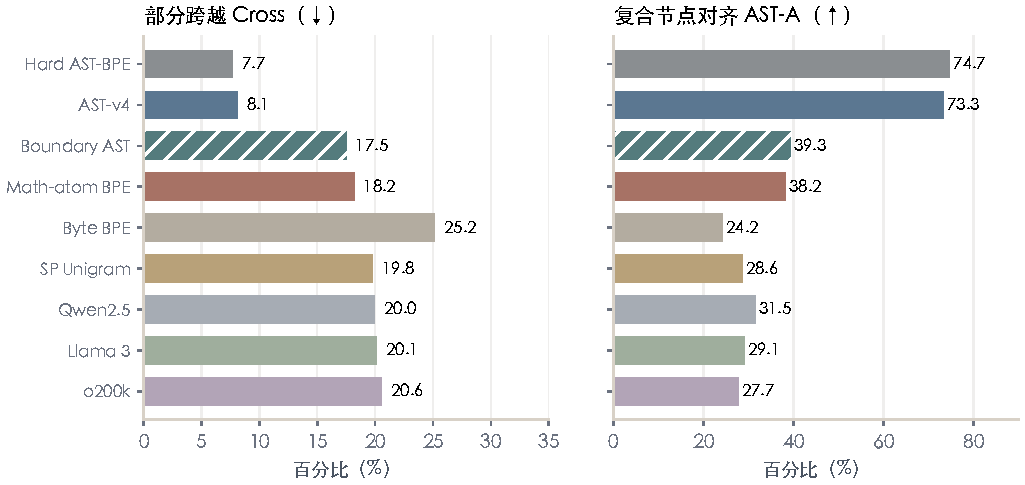
\includegraphics[width=\linewidth]{figures/structure.pdf}\caption{全领域测试中的两种结构测量。柱形为三个来源划分的均值，数值单位为\%。}\label{fig:structure}\end{figure}
\subsection{整域与极限OOD：词表的跨学科迁移}
\par\begin{table}[H]\centering\small
\caption{三个整域留出设置的等权均值。}\label{tab:ood}
\begin{tabular}{lrrrrrrrr}\toprule
模型 & T/B $\dn$ & Cmd $\up$ & Num $\up$ & Cross $\dn$ & AST-A $\up$ & Used & $\eta_{2.5}$ $\up$ & 速度 $\up$ \\\midrule
Hard AST-BPE & 0.4287 & 91.60 & 97.54 & \textbf{7.32} & \textbf{76.29} & 75.88 & 61.52 & 14.67 \\
AST-v4 & 0.4089 & 98.90 & 97.60 & 7.81 & 74.69 & 78.16 & 61.34 & \textbf{30.67} \\
Boundary AST & \textbf{0.3869} & \textbf{99.70} & 97.08 & 17.26 & 40.08 & 71.39 & 69.31 & 27.80 \\
Math-atom BPE & 0.3908 & \textbf{99.70} & 97.08 & 17.79 & 38.81 & 71.48 & 69.65 & 9.39 \\
Byte BPE & 0.4161 & 46.20 & 97.08 & 23.47 & 26.13 & 79.49 & \textbf{74.39} & 7.73 \\
SP Unigram & 0.4890 & 3.09 & 97.92 & 19.49 & 28.77 & 72.56 & 59.76 & 22.57 \\
\midrule
Qwen2.5 & 0.5238 & 2.10 & 97.08 & 19.54 & 32.22 & 1.38 & 33.07 & 3.17 \\
Llama 3 & 0.5211 & 2.10 & \textbf{99.36} & 19.66 & 30.09 & 1.90 & 33.59 & 8.80 \\
o200k & 0.5169 & 2.52 & \textbf{99.36} & 20.04 & 28.99 & 1.19 & 32.81 & 14.01 \\
\bottomrule\end{tabular}
\end{table}\par

\par\begin{table}[H]\centering\small
\caption{分析／方程与代数／数论双向极限OOD的均值。}\label{tab:extreme}
\begin{tabular}{lrrrrrrrr}\toprule
模型 & T/B $\dn$ & Cmd $\up$ & Num $\up$ & Cross $\dn$ & AST-A $\up$ & Used & $\eta_{2.5}$ $\up$ & 速度 $\up$ \\\midrule
Hard AST-BPE & 0.4374 & 87.14 & 96.10 & \textbf{7.30} & \textbf{78.48} & 75.44 & 60.84 & 15.10 \\
AST-v4 & 0.4220 & 98.27 & 96.10 & 7.61 & 77.80 & 76.07 & 59.94 & \textbf{30.72} \\
Boundary AST & \textbf{0.3919} & \textbf{98.58} & 95.29 & 16.59 & 42.90 & 74.61 & 69.38 & 27.98 \\
Math-atom BPE & 0.3967 & \textbf{98.58} & 95.29 & 16.94 & 41.79 & 74.46 & 69.83 & 9.56 \\
Byte BPE & 0.4286 & 45.84 & 95.34 & 21.52 & 31.40 & 77.05 & \textbf{72.69} & 7.71 \\
SP Unigram & 0.5019 & 3.38 & 96.39 & 18.80 & 30.75 & 71.34 & 61.26 & 22.21 \\
\midrule
Qwen2.5 & 0.5265 & 1.95 & 95.28 & 19.22 & 34.52 & 1.40 & 33.21 & 3.13 \\
Llama 3 & 0.5219 & 1.95 & \textbf{99.01} & 19.40 & 30.67 & 1.98 & 33.78 & 8.76 \\
o200k & 0.5183 & 2.54 & \textbf{99.01} & 19.71 & 29.61 & 1.25 & 33.04 & 14.30 \\
\bottomrule\end{tabular}
\end{table}\par

整域 OOD中，T/B最小者为Boundary AST（0.3869）。Boundary AST的Cmd为99.70\%，AST-v4的AST-A为74.69\%。完整留出领域和方向分别列于表\ref{tab:splits}与附录。
极限 OOD中，T/B最小者为Boundary AST（0.3919）。Boundary AST的Cmd为98.58\%，AST-v4的AST-A为77.80\%。完整留出领域和方向分别列于表\ref{tab:splits}与附录。
\subsection{简单到复杂：长度与层次变化}
\par\begin{table}[H]\centering\small
\caption{简单公式训练、复杂公式测试：三个来源划分均值。}\label{tab:complexity}
\begin{tabular}{lrrrrrrrr}\toprule
模型 & T/B $\dn$ & Cmd $\up$ & Num $\up$ & Cross $\dn$ & AST-A $\up$ & Used & $\eta_{2.5}$ $\up$ & 速度 $\up$ \\\midrule
Hard AST-BPE & 0.4226 & 86.17 & 96.91 & \textbf{7.63} & \textbf{74.66} & 73.11 & 61.78 & 16.38 \\
AST-v4 & 0.4022 & 98.81 & 96.93 & 8.06 & 73.25 & 74.25 & 61.87 & \textbf{41.04} \\
Boundary AST & \textbf{0.3802} & \textbf{99.62} & 96.13 & 17.96 & 38.18 & 67.25 & 69.29 & 36.33 \\
Math-atom BPE & 0.3852 & \textbf{99.62} & 96.13 & 19.16 & 36.13 & 67.06 & 69.41 & 11.88 \\
Byte BPE & 0.4084 & 64.80 & 96.13 & 21.50 & 29.17 & 76.89 & \textbf{72.04} & 9.56 \\
SP Unigram & 0.5020 & 2.72 & 97.42 & 16.00 & 37.73 & 67.84 & 53.34 & 29.80 \\
\midrule
Qwen2.5 & 0.5142 & 2.73 & 96.13 & 20.40 & 30.86 & 0.87 & 32.83 & 3.47 \\
Llama 3 & 0.5110 & 2.73 & \textbf{99.14} & 20.58 & 28.38 & 1.09 & 33.37 & 10.12 \\
o200k & 0.5058 & 3.29 & \textbf{99.14} & 21.09 & 26.98 & 0.68 & 32.49 & 16.31 \\
\bottomrule\end{tabular}
\end{table}\par

只在简单公式上构建词表后，Boundary AST在复杂公式上的T/B为0.3802，相对Byte BPE减少6.91\%，Cmd为99.62\%。AST-v4的AST-A为73.25\%，编码速度为41.04 MiB/s。该设置同时改变未见来源与公式句法复杂度。
\begin{figure}[htbp]\centering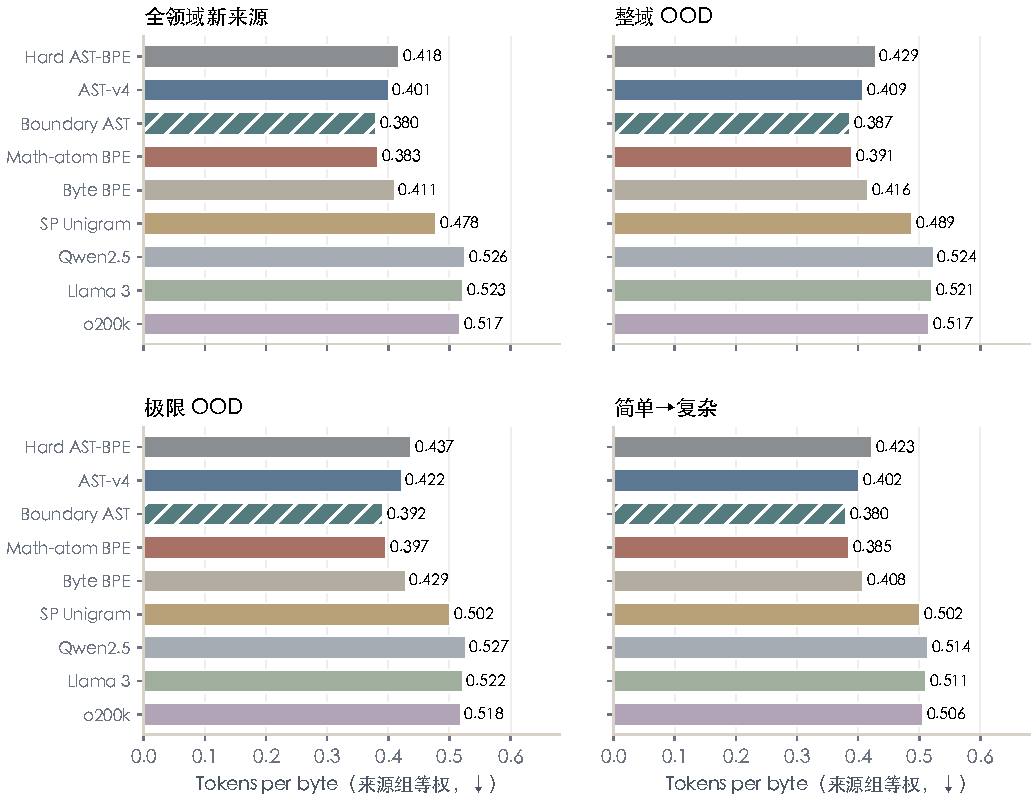
\includegraphics[width=\linewidth]{figures/compression.pdf}\caption{四类泛化测试的压缩结果。各柱为同类设置等权均值；横轴从零开始，越短表示每字节所需token越少。}\label{fig:compression}\end{figure}
\subsection{运行速度与词表使用}
全领域测试中，AST-v4、Boundary AST、Math-atom BPE和Byte BPE的平均完整编码速度分别为32.42、29.36、10.00与8.49 MiB/s。AST-v4和Boundary AST在C前端中融合解析、trie与路径搜索；速度比较涵盖全部这些步骤。Used以完整ID空间为分母，通用词表与数学专用词表在本公式集上的实际使用比例直接列于各表。
\begin{figure}[htbp]\centering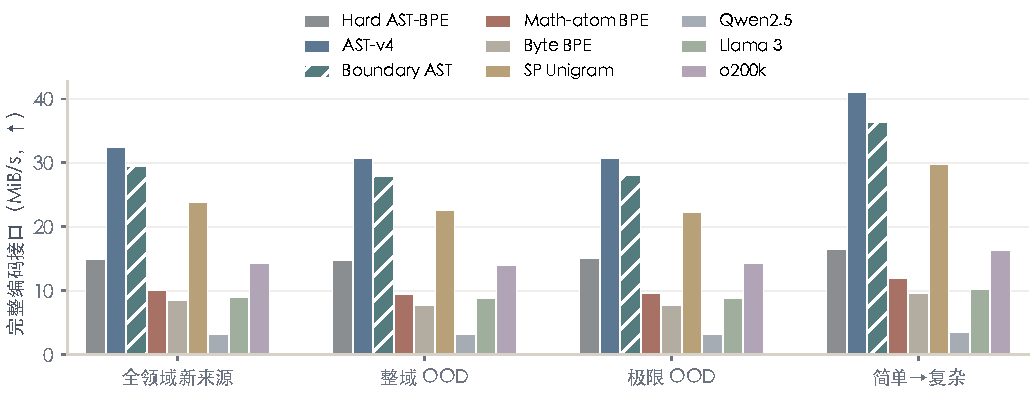
\includegraphics[width=\linewidth]{figures/speed.pdf}\caption{相同测试输入、逐公式完整接口和七轮交错计时下的编码速度。每类对其设置等权平均。}\label{fig:speed}\end{figure}
\subsection{分指标排序与模型选择}
Boundary AST在11个单独设置中均取得最低T/B。以四类测试分别等权后得到分指标前三名，见表\ref{tab:ranks}；数值相同时并列，表格展示顺序沿用模型列表。Used描述测试集使用词表的比例。压缩、命令和数字完整性、语法对齐、分布均匀性与速度分别报告。
\par\begin{table}[H]\centering\small\caption{四类测试等权后的分指标排序，等值并列。Used不用于质量排序。}\label{tab:ranks}\begin{tabularx}{\linewidth}{lYYY}\toprule 指标&第一梯队&第二梯队&第三梯队\\\midrule
T/B & Boundary AST 0.3847 & Math-atom BPE 0.3889 & AST-v4 0.4084 \\
Cmd & Boundary AST／Math-atom BPE 99.41\% & AST-v4 98.75\% & Hard AST-BPE 89.30\% \\
Num & Llama 3／o200k 99.19\% & SP Unigram 97.28\% & AST-v4 96.87\% \\
Cross & Hard AST-BPE 7.49\% & AST-v4 7.89\% & Boundary AST 17.33\% \\
AST-A & Hard AST-BPE 76.04\% & AST-v4 74.77\% & Boundary AST 40.11\% \\
$\eta_{2.5}$ & Byte BPE 73.57\% & Math-atom BPE 69.81\% & Boundary AST 69.42\% \\
速度 & AST-v4 33.71 & Boundary AST 30.37 & SP Unigram 24.59 \\
\bottomrule\end{tabularx}\end{table}\par
下游实验保留软约束Boundary AST与硬约束AST-v4两个结构工作点，以Math-atom BPE分离词表与分割贡献，并保留Byte BPE、SP Unigram及三个通用词表作为参照。标准硬AST-BPE给出不预留数学原子的硬结构基线。


\section{结论与后续实验}
固定1,024词表的实验显示，数学原子能够提高完整命令的表示，结构信号决定压缩与复合节点边界之间的工作点。Boundary AST在全领域新来源测试中取得0.3799的T/B，AST-v4取得73.33\%的复合节点对齐率和32.42 MiB/s的完整编码速度。四类划分将来源泛化、学科迁移与复杂度迁移分开测量，八项指标从压缩、词表使用、结构和运行效率描述各模型。下一阶段将采用相同模型架构、训练字节量和计算预算，从零训练接入不同分词器的模型，评价PDE／ODE求解、符号求导与积分、非方程类数学推理；同时比较训练吞吐、总训练计算量与任务准确率。


\FloatBarrier
\bibliographystyle{unsrtnat}
\bibliography{references}
\clearpage\appendix
\section{各组划分的完整结果}
所有表格采用同一列顺序和相同统计口径。T/B 为来源组等权平均；Cmd、Num、Cross、AST-A、Used 和 $\eta_{2.5}$ 均以百分数表示；速度单位为 MiB/s。每组测试公式完全相同。表中同时列出六个1,024词表模型与三个使用官方完整词表的通用模型。
\par\begin{table}[htbp]\centering\small
\caption{id\_17：训练44,070、验证4,656、测试7,022条公式。}
\begin{tabular}{lrrrrrrrr}\toprule
模型 & T/B $\dn$ & Cmd $\up$ & Num $\up$ & Cross $\dn$ & AST-A $\up$ & Used & $\eta_{2.5}$ $\up$ & 速度 $\up$ \\\midrule
Hard AST-BPE & 0.4253 & 92.92 & 98.14 & \textbf{8.32} & \textbf{73.77} & 75.00 & 62.82 & 14.77 \\
AST-v4 & 0.4094 & 99.07 & 98.14 & 8.61 & 72.66 & 76.27 & 62.27 & \textbf{32.99} \\
Boundary AST & \textbf{0.3829} & \textbf{99.92} & 97.63 & 18.85 & 37.08 & 67.97 & 70.75 & 29.63 \\
Math-atom BPE & 0.3860 & \textbf{99.92} & 97.63 & 19.87 & 35.45 & 68.16 & 71.12 & 10.34 \\
Byte BPE & 0.4152 & 38.04 & 97.63 & 26.31 & 22.16 & 78.71 & \textbf{75.08} & 8.59 \\
SP Unigram & 0.4827 & 4.16 & 98.38 & 20.32 & 27.13 & 71.00 & 59.99 & 25.26 \\
\midrule
Qwen2.5 & 0.5360 & 2.54 & 97.63 & 20.70 & 29.06 & 1.04 & 32.63 & 3.17 \\
Llama 3 & 0.5320 & 2.54 & \textbf{98.67} & 20.81 & 28.07 & 1.31 & 33.14 & 9.05 \\
o200k & 0.5257 & 2.92 & \textbf{98.67} & 21.24 & 26.39 & 0.81 & 32.54 & 14.19 \\
\bottomrule\end{tabular}
\end{table}\par


\par\begin{table}[htbp]\centering\small
\caption{complexity\_17：训练29,863、验证3,032、测试2,769条公式。}
\begin{tabular}{lrrrrrrrr}\toprule
模型 & T/B $\dn$ & Cmd $\up$ & Num $\up$ & Cross $\dn$ & AST-A $\up$ & Used & $\eta_{2.5}$ $\up$ & 速度 $\up$ \\\midrule
Hard AST-BPE & 0.4223 & 83.58 & 98.04 & \textbf{7.82} & \textbf{74.06} & 74.71 & 61.99 & 16.26 \\
AST-v4 & 0.4001 & 99.09 & 98.11 & 8.42 & 72.76 & 75.29 & 62.04 & \textbf{39.21} \\
Boundary AST & \textbf{0.3768} & \textbf{99.86} & 97.36 & 18.46 & 37.00 & 67.77 & 70.16 & 34.97 \\
Math-atom BPE & 0.3822 & \textbf{99.86} & 97.36 & 20.53 & 33.82 & 67.68 & 69.66 & 11.65 \\
Byte BPE & 0.4059 & 67.29 & 97.36 & 21.61 & 28.11 & 78.22 & \textbf{71.65} & 9.44 \\
SP Unigram & 0.5009 & 1.60 & 98.26 & 15.58 & 36.21 & 68.16 & 53.37 & 28.89 \\
\midrule
Qwen2.5 & 0.5219 & 3.27 & 97.36 & 20.90 & 28.64 & 0.90 & 32.51 & 3.43 \\
Llama 3 & 0.5190 & 3.27 & \textbf{98.45} & 20.99 & 27.71 & 1.13 & 33.03 & 10.06 \\
o200k & 0.5123 & 3.68 & \textbf{98.45} & 21.51 & 25.88 & 0.70 & 32.43 & 16.03 \\
\bottomrule\end{tabular}
\end{table}\par


\par\begin{table}[htbp]\centering\small
\caption{id\_29：训练43,262、验证8,317、测试4,184条公式。}
\begin{tabular}{lrrrrrrrr}\toprule
模型 & T/B $\dn$ & Cmd $\up$ & Num $\up$ & Cross $\dn$ & AST-A $\up$ & Used & $\eta_{2.5}$ $\up$ & 速度 $\up$ \\\midrule
Hard AST-BPE & 0.4220 & 91.85 & 95.77 & \textbf{7.05} & \textbf{75.47} & 74.22 & 63.46 & 15.11 \\
AST-v4 & 0.4027 & 98.70 & 95.77 & 7.46 & 74.14 & 76.27 & 63.32 & \textbf{33.97} \\
Boundary AST & \textbf{0.3861} & \textbf{99.37} & 95.43 & 17.57 & 38.26 & 66.80 & 70.28 & 29.70 \\
Math-atom BPE & 0.3894 & \textbf{99.37} & 95.43 & 18.23 & 37.39 & 66.99 & 70.87 & 10.02 \\
Byte BPE & 0.4138 & 38.62 & 95.43 & 25.58 & 23.88 & 76.95 & \textbf{75.50} & 8.75 \\
SP Unigram & 0.4782 & 3.87 & 96.53 & 20.15 & 27.87 & 71.29 & 60.08 & 23.56 \\
\midrule
Qwen2.5 & 0.5304 & 2.02 & 95.43 & 20.19 & 31.72 & 0.89 & 33.29 & 3.12 \\
Llama 3 & 0.5257 & 2.02 & \textbf{99.33} & 20.43 & 27.80 & 1.17 & 33.84 & 9.00 \\
o200k & 0.5206 & 2.36 & \textbf{99.33} & 20.96 & 26.06 & 0.74 & 32.59 & 14.59 \\
\bottomrule\end{tabular}
\end{table}\par


\par\begin{table}[htbp]\centering\small
\caption{complexity\_29：训练29,119、验证5,347、测试1,487条公式。}
\begin{tabular}{lrrrrrrrr}\toprule
模型 & T/B $\dn$ & Cmd $\up$ & Num $\up$ & Cross $\dn$ & AST-A $\up$ & Used & $\eta_{2.5}$ $\up$ & 速度 $\up$ \\\midrule
Hard AST-BPE & 0.4333 & 84.70 & 95.23 & \textbf{6.97} & \textbf{75.84} & 71.19 & 62.02 & 16.71 \\
AST-v4 & 0.4072 & 98.54 & 95.23 & 7.53 & 74.05 & 72.85 & 62.38 & \textbf{41.79} \\
Boundary AST & \textbf{0.3868} & \textbf{99.20} & 94.42 & 18.35 & 36.59 & 65.62 & 69.09 & 36.95 \\
Math-atom BPE & 0.3915 & \textbf{99.20} & 94.42 & 19.31 & 35.61 & 65.23 & 69.29 & 12.12 \\
Byte BPE & 0.4208 & 55.01 & 94.42 & 22.79 & 26.48 & 75.00 & \textbf{71.80} & 9.81 \\
SP Unigram & 0.5096 & 2.50 & 96.11 & 15.85 & 39.47 & 67.29 & 52.42 & 29.88 \\
\midrule
Qwen2.5 & 0.5192 & 2.78 & 94.42 & 20.57 & 31.77 & 0.75 & 33.00 & 3.42 \\
Llama 3 & 0.5136 & 2.78 & \textbf{99.20} & 20.86 & 27.28 & 0.97 & 33.57 & 10.05 \\
o200k & 0.5097 & 2.83 & \textbf{99.20} & 21.45 & 25.49 & 0.61 & 32.38 & 16.30 \\
\bottomrule\end{tabular}
\end{table}\par


\par\begin{table}[htbp]\centering\small
\caption{id\_43：训练44,515、验证5,516、测试5,725条公式。}
\begin{tabular}{lrrrrrrrr}\toprule
模型 & T/B $\dn$ & Cmd $\up$ & Num $\up$ & Cross $\dn$ & AST-A $\up$ & Used & $\eta_{2.5}$ $\up$ & 速度 $\up$ \\\midrule
Hard AST-BPE & 0.4069 & 92.07 & 96.71 & \textbf{7.75} & \textbf{74.88} & 75.00 & 62.36 & 14.54 \\
AST-v4 & 0.3897 & 99.27 & 96.71 & 8.19 & 73.20 & 77.73 & 62.00 & \textbf{30.30} \\
Boundary AST & \textbf{0.3709} & \textbf{99.92} & 96.06 & 16.07 & 42.50 & 69.14 & 68.02 & 28.74 \\
Math-atom BPE & 0.3737 & \textbf{99.92} & 96.06 & 16.44 & 41.85 & 68.95 & 69.09 & 9.65 \\
Byte BPE & 0.4027 & 32.14 & 96.06 & 23.62 & 26.65 & 79.10 & \textbf{74.92} & 8.15 \\
SP Unigram & 0.4741 & 4.52 & 97.34 & 18.93 & 30.66 & 72.66 & 59.79 & 22.47 \\
\midrule
Qwen2.5 & 0.5120 & 1.51 & 96.06 & 19.05 & 33.74 & 1.13 & 33.04 & 3.15 \\
Llama 3 & 0.5106 & 1.51 & \textbf{99.70} & 19.19 & 31.30 & 1.41 & 33.57 & 8.94 \\
o200k & 0.5057 & 2.56 & \textbf{99.70} & 19.53 & 30.78 & 0.87 & 32.76 & 14.05 \\
\bottomrule\end{tabular}
\end{table}\par


\par\begin{table}[htbp]\centering\small
\caption{complexity\_43：训练29,347、验证3,768、测试1,684条公式。}
\begin{tabular}{lrrrrrrrr}\toprule
模型 & T/B $\dn$ & Cmd $\up$ & Num $\up$ & Cross $\dn$ & AST-A $\up$ & Used & $\eta_{2.5}$ $\up$ & 速度 $\up$ \\\midrule
Hard AST-BPE & 0.4121 & 90.23 & 97.45 & \textbf{8.11} & \textbf{74.09} & 73.44 & 61.32 & 16.17 \\
AST-v4 & 0.3992 & 98.81 & 97.45 & 8.23 & 72.95 & 74.61 & 61.20 & \textbf{42.12} \\
Boundary AST & \textbf{0.3771} & \textbf{99.80} & 96.60 & 17.05 & 40.96 & 68.36 & 68.62 & 37.07 \\
Math-atom BPE & 0.3820 & \textbf{99.80} & 96.60 & 17.66 & 38.96 & 68.26 & 69.28 & 11.85 \\
Byte BPE & 0.3985 & 72.12 & 96.60 & 20.10 & 32.93 & 77.44 & \textbf{72.66} & 9.44 \\
SP Unigram & 0.4956 & 4.04 & 97.89 & 16.56 & 37.51 & 68.07 & 54.22 & 30.64 \\
\midrule
Qwen2.5 & 0.5015 & 2.14 & 96.60 & 19.74 & 32.18 & 0.95 & 32.98 & 3.54 \\
Llama 3 & 0.5003 & 2.14 & \textbf{99.78} & 19.90 & 30.14 & 1.17 & 33.51 & 10.25 \\
o200k & 0.4954 & 3.37 & \textbf{99.78} & 20.30 & 29.58 & 0.73 & 32.67 & 16.59 \\
\bottomrule\end{tabular}
\end{table}\par


\par\begin{table}[htbp]\centering\small
\caption{ood\_1：训练31,684、验证5,214、测试18,622条公式。}
\begin{tabular}{lrrrrrrrr}\toprule
模型 & T/B $\dn$ & Cmd $\up$ & Num $\up$ & Cross $\dn$ & AST-A $\up$ & Used & $\eta_{2.5}$ $\up$ & 速度 $\up$ \\\midrule
Hard AST-BPE & 0.4420 & 90.15 & 95.91 & \textbf{6.29} & \textbf{78.62} & 77.25 & 59.95 & 14.61 \\
AST-v4 & 0.4239 & 98.67 & 95.91 & 6.81 & 77.39 & 79.20 & 59.80 & \textbf{27.84} \\
Boundary AST & \textbf{0.4016} & \textbf{99.50} & 95.60 & 17.66 & 40.73 & 74.51 & 68.51 & 25.80 \\
Math-atom BPE & 0.4047 & \textbf{99.50} & 95.60 & 18.36 & 39.48 & 74.51 & 68.93 & 8.54 \\
Byte BPE & 0.4305 & 26.77 & 95.60 & 23.81 & 27.33 & 79.98 & \textbf{73.77} & 7.09 \\
SP Unigram & 0.4919 & 3.40 & 96.37 & 20.11 & 29.37 & 73.93 & 61.38 & 20.52 \\
\midrule
Qwen2.5 & 0.5330 & 2.18 & 95.60 & 19.92 & 34.47 & 1.52 & 33.36 & 3.03 \\
Llama 3 & 0.5281 & 2.18 & \textbf{99.31} & 20.11 & 30.46 & 2.27 & 33.92 & 8.41 \\
o200k & 0.5251 & 2.79 & \textbf{99.31} & 20.37 & 29.74 & 1.43 & 33.27 & 13.44 \\
\bottomrule\end{tabular}
\end{table}\par


\par\begin{table}[htbp]\centering\small
\caption{ood\_2：训练42,081、验证6,357、测试7,334条公式。}
\begin{tabular}{lrrrrrrrr}\toprule
模型 & T/B $\dn$ & Cmd $\up$ & Num $\up$ & Cross $\dn$ & AST-A $\up$ & Used & $\eta_{2.5}$ $\up$ & 速度 $\up$ \\\midrule
Hard AST-BPE & 0.4305 & 91.04 & 98.80 & \textbf{7.85} & \textbf{75.20} & 74.32 & 62.57 & 14.87 \\
AST-v4 & 0.4050 & 98.98 & 98.95 & 8.26 & 73.38 & 76.86 & 62.27 & \textbf{33.33} \\
Boundary AST & \textbf{0.3831} & \textbf{99.81} & 98.26 & 16.90 & 39.30 & 69.24 & 69.66 & 29.41 \\
Math-atom BPE & 0.3881 & \textbf{99.81} & 98.26 & 17.30 & 38.02 & 69.34 & 69.89 & 10.46 \\
Byte BPE & 0.4138 & 53.05 & 98.26 & 23.57 & 24.18 & 79.00 & \textbf{74.99} & 8.70 \\
SP Unigram & 0.4990 & 2.14 & 99.06 & 18.79 & 27.20 & 71.09 & 58.57 & 24.58 \\
\midrule
Qwen2.5 & 0.5148 & 2.21 & 98.26 & 18.86 & 31.52 & 1.11 & 32.95 & 3.29 \\
Llama 3 & 0.5142 & 2.21 & \textbf{99.52} & 18.91 & 30.78 & 1.35 & 33.43 & 9.08 \\
o200k & 0.5111 & 1.81 & \textbf{99.52} & 19.43 & 29.32 & 0.84 & 32.46 & 14.56 \\
\bottomrule\end{tabular}
\end{table}\par


\par\begin{table}[htbp]\centering\small
\caption{ood\_3：训练31,313、验证4,022、测试20,259条公式。}
\begin{tabular}{lrrrrrrrr}\toprule
模型 & T/B $\dn$ & Cmd $\up$ & Num $\up$ & Cross $\dn$ & AST-A $\up$ & Used & $\eta_{2.5}$ $\up$ & 速度 $\up$ \\\midrule
Hard AST-BPE & 0.4136 & 93.61 & 97.91 & \textbf{7.83} & \textbf{75.03} & 76.07 & 62.03 & 14.53 \\
AST-v4 & 0.3977 & 99.06 & 97.93 & 8.37 & 73.30 & 78.42 & 61.94 & \textbf{30.84} \\
Boundary AST & \textbf{0.3759} & \textbf{99.78} & 97.37 & 17.23 & 40.19 & 70.41 & 69.77 & 28.18 \\
Math-atom BPE & 0.3796 & \textbf{99.78} & 97.37 & 17.72 & 38.93 & 70.61 & 70.11 & 9.16 \\
Byte BPE & 0.4040 & 58.77 & 97.37 & 23.03 & 26.87 & 79.49 & \textbf{74.41} & 7.40 \\
SP Unigram & 0.4761 & 3.73 & 98.33 & 19.56 & 29.74 & 72.66 & 59.35 & 22.63 \\
\midrule
Qwen2.5 & 0.5236 & 1.91 & 97.37 & 19.86 & 30.67 & 1.52 & 32.92 & 3.18 \\
Llama 3 & 0.5209 & 1.91 & \textbf{99.27} & 19.96 & 29.03 & 2.07 & 33.41 & 8.89 \\
o200k & 0.5144 & 2.94 & \textbf{99.27} & 20.32 & 27.92 & 1.31 & 32.71 & 14.04 \\
\bottomrule\end{tabular}
\end{table}\par


\par\begin{table}[htbp]\centering\small
\caption{extreme\_analysis\_equations\_to\_algebra：训练16,893、验证3,298、测试8,576条公式。}
\begin{tabular}{lrrrrrrrr}\toprule
模型 & T/B $\dn$ & Cmd $\up$ & Num $\up$ & Cross $\dn$ & AST-A $\up$ & Used & $\eta_{2.5}$ $\up$ & 速度 $\up$ \\\midrule
Hard AST-BPE & 0.4503 & 85.90 & 93.90 & \textbf{7.20} & \textbf{79.49} & 74.12 & 60.90 & 15.15 \\
AST-v4 & 0.4351 & 98.62 & 93.90 & 7.51 & 78.82 & 75.59 & 59.90 & \textbf{30.18} \\
Boundary AST & \textbf{0.4015} & \textbf{98.93} & 93.19 & 16.12 & 44.88 & 74.90 & 69.74 & 27.82 \\
Math-atom BPE & 0.4061 & \textbf{98.93} & 93.19 & 16.42 & 44.12 & 74.80 & 70.07 & 9.77 \\
Byte BPE & 0.4396 & 54.39 & 93.19 & 19.66 & 36.45 & 76.86 & \textbf{72.82} & 8.02 \\
SP Unigram & 0.5124 & 2.45 & 94.21 & 18.10 & 33.75 & 70.90 & 61.64 & 21.87 \\
\midrule
Qwen2.5 & 0.5294 & 1.98 & 93.19 & 18.59 & 38.34 & 1.28 & 33.51 & 3.07 \\
Llama 3 & 0.5228 & 1.98 & \textbf{98.76} & 18.86 & 32.27 & 1.88 & 34.15 & 8.62 \\
o200k & 0.5221 & 2.15 & \textbf{98.76} & 19.11 & 31.27 & 1.19 & 33.38 & 14.24 \\
\bottomrule\end{tabular}
\end{table}\par


\par\begin{table}[htbp]\centering\small
\caption{extreme\_algebra\_to\_analysis\_equations：训练7,707、验证1,002、测试20,420条公式。}
\begin{tabular}{lrrrrrrrr}\toprule
模型 & T/B $\dn$ & Cmd $\up$ & Num $\up$ & Cross $\dn$ & AST-A $\up$ & Used & $\eta_{2.5}$ $\up$ & 速度 $\up$ \\\midrule
Hard AST-BPE & 0.4246 & 88.38 & 98.30 & \textbf{7.39} & \textbf{77.47} & 76.76 & 60.78 & 15.05 \\
AST-v4 & 0.4089 & 97.93 & 98.30 & 7.70 & 76.79 & 76.56 & 59.98 & \textbf{31.26} \\
Boundary AST & \textbf{0.3824} & \textbf{98.22} & 97.40 & 17.06 & 40.92 & 74.32 & 69.01 & 28.14 \\
Math-atom BPE & 0.3873 & \textbf{98.22} & 97.40 & 17.46 & 39.46 & 74.12 & 69.60 & 9.35 \\
Byte BPE & 0.4175 & 37.30 & 97.50 & 23.39 & 26.36 & 77.25 & \textbf{72.56} & 7.39 \\
SP Unigram & 0.4914 & 4.31 & 98.56 & 19.50 & 27.75 & 71.78 & 60.88 & 22.55 \\
\midrule
Qwen2.5 & 0.5236 & 1.91 & 97.37 & 19.84 & 30.70 & 1.52 & 32.91 & 3.19 \\
Llama 3 & 0.5210 & 1.91 & \textbf{99.27} & 19.95 & 29.07 & 2.07 & 33.41 & 8.91 \\
o200k & 0.5145 & 2.94 & \textbf{99.27} & 20.30 & 27.95 & 1.31 & 32.70 & 14.36 \\
\bottomrule\end{tabular}
\end{table}\par

\FloatBarrier
\section{实现、复现与审查记录}
代码、数据及全部输出位于\href{https://github.com/xtr1976536/math-tokenizer-lab}{GitHub仓库}。按下列顺序执行实验、复算和报告生成：
\begin{quote}\small\ttfamily
.venv/bin/python scripts/run\_intrinsic\_2026.py\\
.venv/bin/python scripts/audit\_intrinsic\_2026.py\\
.venv/bin/python scripts/build\_intrinsic\_2026\_report.py
\end{quote}
实验目录为\code{experiments/intrinsic_20261015}；协议保存所有训练／验证／测试ID、固定参数、代码哈希、数据哈希与环境信息；每组保存训练所得模型、七轮计时、逐式token ID及统计量。

审查分五轮执行。第一轮检查ID、来源、模板、渲染隔离及领域／复杂度条件；第二轮检查1,024实际ID预算、软约束与数学原子共享词表、硬AST原生实现与独立参考实现的一致性；第三轮检查所有测试公式的精确负载、完整解码、ID范围和七轮确定性；第四轮独立重聚合逐式计数与来源组等权T/B；第五轮从存档token与检查点重建边界，复算所有模型的命令、数字与复合节点对齐，抽样以直接区间判据复核Cross，并调用公开Rényi熵函数核对99组分布统计。所有检查均通过。

独立审查覆盖882,738条模型—公式记录。依赖版本为tokenizers 0.23.3，sentencepiece 0.2.2，tiktoken 0.14.0，numpy 2.4.6，matplotlib 3.11.2。

\subsection{来源组级抽样区间}\begin{table}[htbp]\centering\small\caption{全领域测试T/B及来源组级bootstrap的95\%区间。每个单元第一行为点估计，第二行为区间；三列分别为三个来源划分。}\begin{tabular}{lccc}\toprule 模型&ID-17&ID-29&ID-43\\\midrule
Hard AST-BPE & \shortstack{0.4253\\{}[0.3988, 0.4520]} & \shortstack{0.4220\\{}[0.3965, 0.4490]} & \shortstack{0.4069\\{}[0.3856, 0.4272]} \\
AST-v4 & \shortstack{0.4094\\{}[0.3843, 0.4360]} & \shortstack{0.4027\\{}[0.3788, 0.4290]} & \shortstack{0.3897\\{}[0.3703, 0.4086]} \\
Boundary AST & \shortstack{0.3829\\{}[0.3602, 0.4063]} & \shortstack{0.3861\\{}[0.3648, 0.4083]} & \shortstack{0.3709\\{}[0.3530, 0.3887]} \\
Math-atom BPE & \shortstack{0.3860\\{}[0.3635, 0.4095]} & \shortstack{0.3894\\{}[0.3682, 0.4116]} & \shortstack{0.3737\\{}[0.3558, 0.3918]} \\
Byte BPE & \shortstack{0.4152\\{}[0.3927, 0.4379]} & \shortstack{0.4138\\{}[0.3925, 0.4355]} & \shortstack{0.4027\\{}[0.3840, 0.4204]} \\
SP Unigram & \shortstack{0.4827\\{}[0.4636, 0.5020]} & \shortstack{0.4782\\{}[0.4598, 0.4957]} & \shortstack{0.4741\\{}[0.4576, 0.4898]} \\
Qwen2.5 & \shortstack{0.5360\\{}[0.5201, 0.5526]} & \shortstack{0.5304\\{}[0.5183, 0.5445]} & \shortstack{0.5120\\{}[0.4985, 0.5263]} \\
Llama 3 & \shortstack{0.5320\\{}[0.5155, 0.5491]} & \shortstack{0.5257\\{}[0.5137, 0.5394]} & \shortstack{0.5106\\{}[0.4969, 0.5250]} \\
o200k & \shortstack{0.5257\\{}[0.5073, 0.5452]} & \shortstack{0.5206\\{}[0.5080, 0.5350]} & \shortstack{0.5057\\{}[0.4907, 0.5219]} \\
\bottomrule\end{tabular}\end{table}

\end{document}
